\documentclass{beamer}
\usepackage{graphicx}
\usepackage{listings}
\usepackage{tikz}

\usetheme{Boadilla}
\setlength{\parskip}{\baselineskip}

\title{Range Queries Con Updates}
\subtitle{Segment Tree y otras variantes}
\author{Ulises López Pacholczak}
\date{\today}

\definecolor{keywords}{HTML}{44548A}
\definecolor{strings}{HTML}{00999A}
\definecolor{comments}{HTML}{990000}

\lstset{language=C++,frame=single,basicstyle=\ttfamily \small,showstringspaces=false,columns=flexible}
\lstset{
  literate={ö}{{\"o}}1
           {ä}{{\"a}}1
           {ü}{{\"u}}1
}
\lstset{xleftmargin=0pt,xrightmargin=0pt}
\lstset{aboveskip=12pt,belowskip=8pt}

\lstset{
    commentstyle=\color{comments},
    keywordstyle=\color{keywords},
    stringstyle=\color{strings}
}



\begin{document}

\begin{frame}
\titlepage
\end{frame}

\begin{frame}
\tableofcontents
\end{frame}

\section{Introducción}

\begin{frame}{Introducción}
Ya sabemos como responder queries de suma en rango, en $O(n)$ tiempo de procesamiento ($O(n*m)$ si es una tabla) y $O(1)$ tiempo de consulta.

\pause
También, se pueden resolver queries de máximo o mínimo en rangos con $O(n\:log\: n)$ tiempo de procesamiento y $O(1)$ tiempo de consulta.

\pause
¿Pero esto es suficiente para todos los problemas?
\end{frame}

\section{Segment Tree}

\begin{frame}{Suma en Rangos con Updates}

\begin{block}{CSES 1648 - Dynamic Range Sum Queries}
Dado un arreglo de $n$ enteros, tu tarea es procesar $q$ queries de los siguientes tipos:
\begin{enumerate}
    \item Actualizar el valor en la posición $k$ a un valor $u$
    \item Cual es la suma de los valores en el rango $[a,b]$?
\end{enumerate}
Tanto $q$ y $n$ pueden ser como máximo $2*10^5$
\end{block}

\url{https://cses.fi/problemset/task/1648}
\end{frame}

\begin{frame}{Con lo que ya sabemos...}
Por cada query de tipo $1$, debemos realizar un reprocesamiento de $O(n)$. Por ende, la complejidad del problema nos quedaría $O(n^2)$, lo mismo que hacerlo con fuerza bruta.

\pause
Es claro que necesitamos otra estructura de datos para poder manejar los updates de forma eficiente...
\end{frame}

\subsection{Explicación de la Estructura}
\begin{frame}{Segment Tree}
El Segment Tree es una estructura de datos que nos permite realizar queries en rangos y updates en $O(log\:n)$.
\pause

\begin{center}
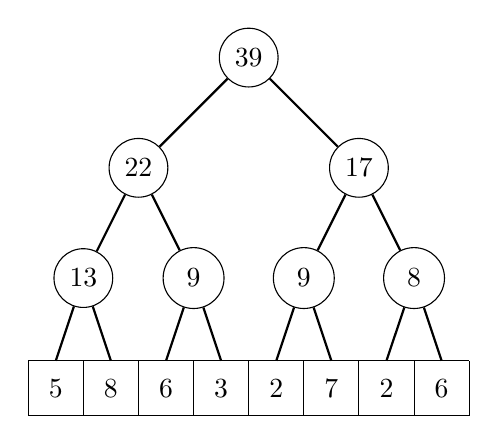
\begin{tikzpicture}[scale=0.7]
\draw (0,0) grid (8,1);

\node[anchor=center] at (0.5, 0.5) {5};
\node[anchor=center] at (1.5, 0.5) {8};
\node[anchor=center] at (2.5, 0.5) {6};
\node[anchor=center] at (3.5, 0.5) {3};
\node[anchor=center] at (4.5, 0.5) {2};
\node[anchor=center] at (5.5, 0.5) {7};
\node[anchor=center] at (6.5, 0.5) {2};
\node[anchor=center] at (7.5, 0.5) {6};

\node[draw, circle] (a) at (1,2.5) {13};
\path[draw,thick,-] (a) -- (0.5,1);
\path[draw,thick,-] (a) -- (1.5,1);
\node[draw, circle,minimum size=22pt] (b) at (3,2.5) {9};
\path[draw,thick,-] (b) -- (2.5,1);
\path[draw,thick,-] (b) -- (3.5,1);
\node[draw, circle,minimum size=22pt] (c) at (5,2.5) {9};
\path[draw,thick,-] (c) -- (4.5,1);
\path[draw,thick,-] (c) -- (5.5,1);
\node[draw, circle,minimum size=22pt] (d) at (7,2.5) {8};
\path[draw,thick,-] (d) -- (6.5,1);
\path[draw,thick,-] (d) -- (7.5,1);

\node[draw, circle] (i) at (2,4.5) {22};
\path[draw,thick,-] (i) -- (a);
\path[draw,thick,-] (i) -- (b);
\node[draw, circle] (j) at (6,4.5) {17};
\path[draw,thick,-] (j) -- (c);
\path[draw,thick,-] (j) -- (d);

\node[draw, circle] (m) at (4,6.5) {39};
\path[draw,thick,-] (m) -- (i);
\path[draw,thick,-] (m) -- (j);
\end{tikzpicture}
\end{center}

\end{frame}

\begin{frame}{Funcionamiento}
Cada nodo representa el valor de realizar una operación (en el caso del problema original, la suma) en un rango del arreglo.

\begin{center}
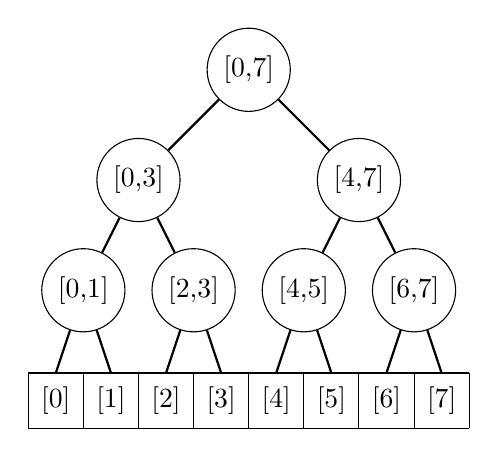
\begin{tikzpicture}[scale=0.7]
%\fill[color=lightgray] (1,0) rectangle (7,1);
\draw (0,0) grid (8,1);

\node[anchor=center] at (0.5, 0.5) {[0]};
\node[anchor=center] at (1.5, 0.5) {[1]};
\node[anchor=center] at (2.5, 0.5) {[2]};
\node[anchor=center] at (3.5, 0.5) {[3]};
\node[anchor=center] at (4.5, 0.5) {[4]};
\node[anchor=center] at (5.5, 0.5) {[5]};
\node[anchor=center] at (6.5, 0.5) {[6]};
\node[anchor=center] at (7.5, 0.5) {[7]};

%fill=lightgray
\node[draw, circle] (a) at (1,2.5) {[0,1]};
\path[draw,thick,-] (a) -- (0.5,1);
\path[draw,thick,-] (a) -- (1.5,1);
\node[draw, circle,minimum size=22pt] (b) at (3,2.5) {[2,3]};
\path[draw,thick,-] (b) -- (2.5,1);
\path[draw,thick,-] (b) -- (3.5,1);
\node[draw, circle,minimum size=22pt] (c) at (5,2.5) {[4,5]};
\path[draw,thick,-] (c) -- (4.5,1);
\path[draw,thick,-] (c) -- (5.5,1);
\node[draw, circle,minimum size=22pt] (d) at (7,2.5) {[6,7]};
\path[draw,thick,-] (d) -- (6.5,1);
\path[draw,thick,-] (d) -- (7.5,1);

\node[draw, circle] (i) at (2,4.5) {[0,3]};
\path[draw,thick,-] (i) -- (a);
\path[draw,thick,-] (i) -- (b);
\node[draw, circle] (j) at (6,4.5) {[4,7]};
\path[draw,thick,-] (j) -- (c);
\path[draw,thick,-] (j) -- (d);

\node[draw, circle] (m) at (4,6.5) {[0,7]};
\path[draw,thick,-] (m) -- (i);
\path[draw,thick,-] (m) -- (j);
\end{tikzpicture}
\end{center}
\end{frame}

\subsection{Ejemplos de Queries y Updates}

\begin{frame}{Guardado de Segment Tree en Memoria}
\begin{center}
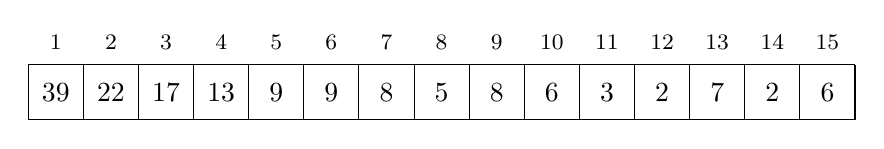
\begin{tikzpicture}[scale=0.7]
\draw (0,0) grid (15,1);

\node at (0.5,0.5) {$39$};
\node at (1.5,0.5) {$22$};
\node at (2.5,0.5) {$17$};
\node at (3.5,0.5) {$13$};
\node at (4.5,0.5) {$9$};
\node at (5.5,0.5) {$9$};
\node at (6.5,0.5) {$8$};
\node at (7.5,0.5) {$5$};
\node at (8.5,0.5) {$8$};
\node at (9.5,0.5) {$6$};
\node at (10.5,0.5) {$3$};
\node at (11.5,0.5) {$2$};
\node at (12.5,0.5) {$7$};
\node at (13.5,0.5) {$2$};
\node at (14.5,0.5) {$6$};

\footnotesize
\node at (0.5,1.4) {$1$};
\node at (1.5,1.4) {$2$};
\node at (2.5,1.4) {$3$};
\node at (3.5,1.4) {$4$};
\node at (4.5,1.4) {$5$};
\node at (5.5,1.4) {$6$};
\node at (6.5,1.4) {$7$};
\node at (7.5,1.4) {$8$};
\node at (8.5,1.4) {$9$};
\node at (9.5,1.4) {$10$};
\node at (10.5,1.4) {$11$};
\node at (11.5,1.4) {$12$};
\node at (12.5,1.4) {$13$};
\node at (13.5,1.4) {$14$};
\node at (14.5,1.4) {$15$};
\end{tikzpicture}
\end{center}
\end{frame}

\begin{frame}{Ejemplo de Query}
\begin{center}
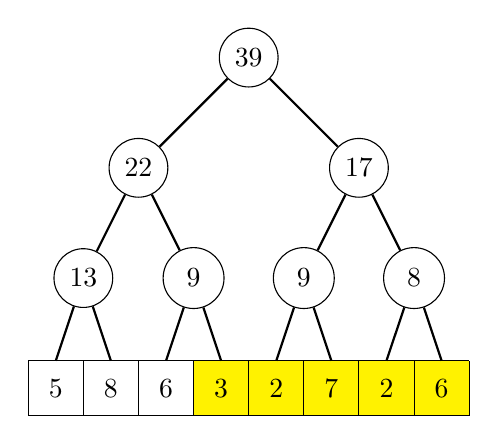
\begin{tikzpicture}[scale=0.7]
\fill[color=yellow] (3,0) rectangle (8,1);
\draw (0,0) grid (8,1);

\node[anchor=center] at (0.5, 0.5) {5};
\node[anchor=center] at (1.5, 0.5) {8};
\node[anchor=center] at (2.5, 0.5) {6};
\node[anchor=center] at (3.5, 0.5) {3};
\node[anchor=center] at (4.5, 0.5) {2};
\node[anchor=center] at (5.5, 0.5) {7};
\node[anchor=center] at (6.5, 0.5) {2};
\node[anchor=center] at (7.5, 0.5) {6};

\node[draw, circle] (a) at (1,2.5) {13};
\path[draw,thick,-] (a) -- (0.5,1);
\path[draw,thick,-] (a) -- (1.5,1);
\node[draw, circle,minimum size=22pt] (b) at (3,2.5) {9};
\path[draw,thick,-] (b) -- (2.5,1);
\path[draw,thick,-] (b) -- (3.5,1);
\node[draw, circle,minimum size=22pt] (c) at (5,2.5) {9};
\path[draw,thick,-] (c) -- (4.5,1);
\path[draw,thick,-] (c) -- (5.5,1);
\node[draw, circle,minimum size=22pt] (d) at (7,2.5) {8};
\path[draw,thick,-] (d) -- (6.5,1);
\path[draw,thick,-] (d) -- (7.5,1);

\node[draw, circle] (i) at (2,4.5) {22};
\path[draw,thick,-] (i) -- (a);
\path[draw,thick,-] (i) -- (b);
\node[draw, circle] (j) at (6,4.5) {17};
\path[draw,thick,-] (j) -- (c);
\path[draw,thick,-] (j) -- (d);

\node[draw, circle] (m) at (4,6.5) {39};
\path[draw,thick,-] (m) -- (i);
\path[draw,thick,-] (m) -- (j);
\end{tikzpicture}
\end{center}
Suma total $= 0$
\end{frame}

\begin{frame}{Ejemplo de Query}
\begin{center}
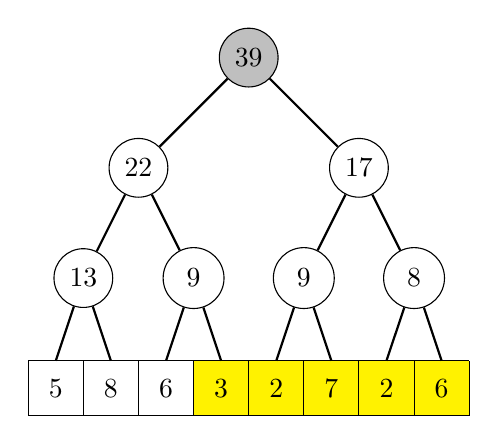
\begin{tikzpicture}[scale=0.7]
\fill[color=yellow] (3,0) rectangle (8,1);
\draw (0,0) grid (8,1);

\node[anchor=center] at (0.5, 0.5) {5};
\node[anchor=center] at (1.5, 0.5) {8};
\node[anchor=center] at (2.5, 0.5) {6};
\node[anchor=center] at (3.5, 0.5) {3};
\node[anchor=center] at (4.5, 0.5) {2};
\node[anchor=center] at (5.5, 0.5) {7};
\node[anchor=center] at (6.5, 0.5) {2};
\node[anchor=center] at (7.5, 0.5) {6};

\node[draw, circle] (a) at (1,2.5) {13};
\path[draw,thick,-] (a) -- (0.5,1);
\path[draw,thick,-] (a) -- (1.5,1);
\node[draw, circle,minimum size=22pt] (b) at (3,2.5) {9};
\path[draw,thick,-] (b) -- (2.5,1);
\path[draw,thick,-] (b) -- (3.5,1);
\node[draw, circle,minimum size=22pt] (c) at (5,2.5) {9};
\path[draw,thick,-] (c) -- (4.5,1);
\path[draw,thick,-] (c) -- (5.5,1);
\node[draw, circle,minimum size=22pt] (d) at (7,2.5) {8};
\path[draw,thick,-] (d) -- (6.5,1);
\path[draw,thick,-] (d) -- (7.5,1);

\node[draw, circle] (i) at (2,4.5) {22};
\path[draw,thick,-] (i) -- (a);
\path[draw,thick,-] (i) -- (b);
\node[draw, circle] (j) at (6,4.5) {17};
\path[draw,thick,-] (j) -- (c);
\path[draw,thick,-] (j) -- (d);

\node[draw, circle,fill=lightgray] (m) at (4,6.5) {39};
\path[draw,thick,-] (m) -- (i);
\path[draw,thick,-] (m) -- (j);
\end{tikzpicture}
\end{center}
Suma total $= 0$
\end{frame}

\begin{frame}{Ejemplo de Query}
\begin{center}
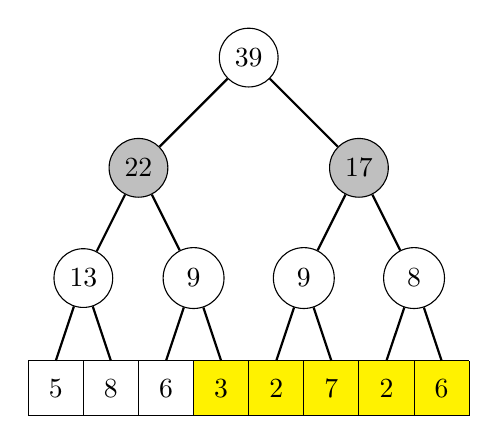
\begin{tikzpicture}[scale=0.7]
\fill[color=yellow] (3,0) rectangle (8,1);
\draw (0,0) grid (8,1);

\node[anchor=center] at (0.5, 0.5) {5};
\node[anchor=center] at (1.5, 0.5) {8};
\node[anchor=center] at (2.5, 0.5) {6};
\node[anchor=center] at (3.5, 0.5) {3};
\node[anchor=center] at (4.5, 0.5) {2};
\node[anchor=center] at (5.5, 0.5) {7};
\node[anchor=center] at (6.5, 0.5) {2};
\node[anchor=center] at (7.5, 0.5) {6};

\node[draw, circle] (a) at (1,2.5) {13};
\path[draw,thick,-] (a) -- (0.5,1);
\path[draw,thick,-] (a) -- (1.5,1);
\node[draw, circle,minimum size=22pt] (b) at (3,2.5) {9};
\path[draw,thick,-] (b) -- (2.5,1);
\path[draw,thick,-] (b) -- (3.5,1);
\node[draw, circle,minimum size=22pt] (c) at (5,2.5) {9};
\path[draw,thick,-] (c) -- (4.5,1);
\path[draw,thick,-] (c) -- (5.5,1);
\node[draw, circle,minimum size=22pt] (d) at (7,2.5) {8};
\path[draw,thick,-] (d) -- (6.5,1);
\path[draw,thick,-] (d) -- (7.5,1);

\node[draw, circle, fill=lightgray] (i) at (2,4.5) {22};
\path[draw,thick,-] (i) -- (a);
\path[draw,thick,-] (i) -- (b);
\node[draw, circle, fill=lightgray] (j) at (6,4.5) {17};
\path[draw,thick,-] (j) -- (c);
\path[draw,thick,-] (j) -- (d);

\node[draw, circle] (m) at (4,6.5) {39};
\path[draw,thick,-] (m) -- (i);
\path[draw,thick,-] (m) -- (j);
\end{tikzpicture}
\end{center}
Suma total $= 0$
\end{frame}

\begin{frame}{Ejemplo de Query}
\begin{center}
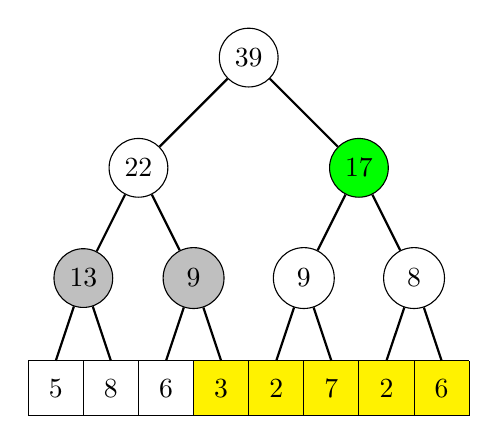
\begin{tikzpicture}[scale=0.7]
\fill[color=yellow] (3,0) rectangle (8,1);
\draw (0,0) grid (8,1);

\node[anchor=center] at (0.5, 0.5) {5};
\node[anchor=center] at (1.5, 0.5) {8};
\node[anchor=center] at (2.5, 0.5) {6};
\node[anchor=center] at (3.5, 0.5) {3};
\node[anchor=center] at (4.5, 0.5) {2};
\node[anchor=center] at (5.5, 0.5) {7};
\node[anchor=center] at (6.5, 0.5) {2};
\node[anchor=center] at (7.5, 0.5) {6};

\node[draw, circle, fill=lightgray] (a) at (1,2.5) {13};
\path[draw,thick,-] (a) -- (0.5,1);
\path[draw,thick,-] (a) -- (1.5,1);
\node[draw, circle, minimum size=22pt, fill=lightgray] (b) at (3,2.5) {9};
\path[draw,thick,-] (b) -- (2.5,1);
\path[draw,thick,-] (b) -- (3.5,1);
\node[draw, circle,minimum size=22pt] (c) at (5,2.5) {9};
\path[draw,thick,-] (c) -- (4.5,1);
\path[draw,thick,-] (c) -- (5.5,1);
\node[draw, circle,minimum size=22pt] (d) at (7,2.5) {8};
\path[draw,thick,-] (d) -- (6.5,1);
\path[draw,thick,-] (d) -- (7.5,1);

\node[draw, circle] (i) at (2,4.5) {22};
\path[draw,thick,-] (i) -- (a);
\path[draw,thick,-] (i) -- (b);
\node[draw, circle, fill=green] (j) at (6,4.5) {17};
\path[draw,thick,-] (j) -- (c);
\path[draw,thick,-] (j) -- (d);

\node[draw, circle] (m) at (4,6.5) {39};
\path[draw,thick,-] (m) -- (i);
\path[draw,thick,-] (m) -- (j);
\end{tikzpicture}
\end{center}
Suma total $= 17$
\end{frame}

\begin{frame}{Ejemplo de Query}
\begin{center}
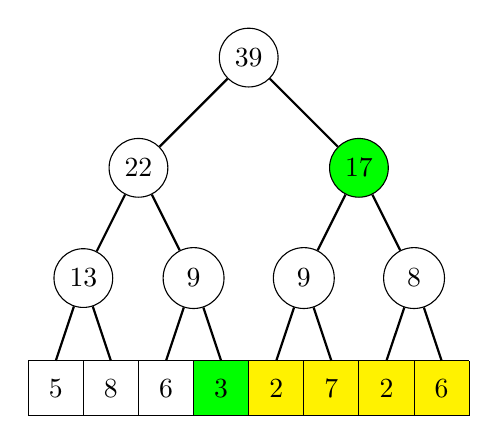
\begin{tikzpicture}[scale=0.7]
\fill[color=green] (3,0) rectangle (4,1);
\draw (0,0) grid (8,1);
\fill[color=yellow] (4,0) rectangle (8,1);
\draw (0,0) grid (8,1);

\node[anchor=center] at (0.5, 0.5) {5};
\node[anchor=center] at (1.5, 0.5) {8};
\node[anchor=center] at (2.5, 0.5) {6};
\node[anchor=center] at (3.5, 0.5) {3};
\node[anchor=center] at (4.5, 0.5) {2};
\node[anchor=center] at (5.5, 0.5) {7};
\node[anchor=center] at (6.5, 0.5) {2};
\node[anchor=center] at (7.5, 0.5) {6};

\node[draw, circle] (a) at (1,2.5) {13};
\path[draw,thick,-] (a) -- (0.5,1);
\path[draw,thick,-] (a) -- (1.5,1);
\node[draw, circle, minimum size=22pt] (b) at (3,2.5) {9};
\path[draw,thick,-] (b) -- (2.5,1);
\path[draw,thick,-] (b) -- (3.5,1);
\node[draw, circle,minimum size=22pt] (c) at (5,2.5) {9};
\path[draw,thick,-] (c) -- (4.5,1);
\path[draw,thick,-] (c) -- (5.5,1);
\node[draw, circle,minimum size=22pt] (d) at (7,2.5) {8};
\path[draw,thick,-] (d) -- (6.5,1);
\path[draw,thick,-] (d) -- (7.5,1);

\node[draw, circle] (i) at (2,4.5) {22};
\path[draw,thick,-] (i) -- (a);
\path[draw,thick,-] (i) -- (b);
\node[draw, circle, fill=green] (j) at (6,4.5) {17};
\path[draw,thick,-] (j) -- (c);
\path[draw,thick,-] (j) -- (d);

\node[draw, circle] (m) at (4,6.5) {39};
\path[draw,thick,-] (m) -- (i);
\path[draw,thick,-] (m) -- (j);
\end{tikzpicture}
\end{center}
Suma total $= 20$
\end{frame}

\begin{frame}{Ejemplo de Update}
\begin{center}
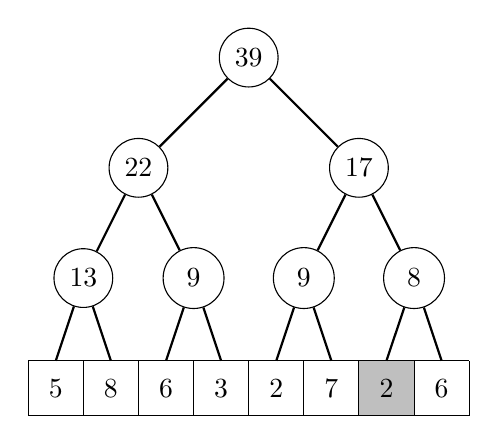
\begin{tikzpicture}[scale=0.7]
\fill[color=lightgray] (6,0) rectangle (7,1);
\draw (0,0) grid (8,1);

\node[anchor=center] at (0.5, 0.5) {5};
\node[anchor=center] at (1.5, 0.5) {8};
\node[anchor=center] at (2.5, 0.5) {6};
\node[anchor=center] at (3.5, 0.5) {3};
\node[anchor=center] at (4.5, 0.5) {2};
\node[anchor=center] at (5.5, 0.5) {7};
\node[anchor=center] at (6.5, 0.5) {2};
\node[anchor=center] at (7.5, 0.5) {6};

\node[draw, circle] (a) at (1,2.5) {13};
\path[draw,thick,-] (a) -- (0.5,1);
\path[draw,thick,-] (a) -- (1.5,1);
\node[draw, circle,minimum size=22pt] (b) at (3,2.5) {9};
\path[draw,thick,-] (b) -- (2.5,1);
\path[draw,thick,-] (b) -- (3.5,1);
\node[draw, circle,minimum size=22pt] (c) at (5,2.5) {9};
\path[draw,thick,-] (c) -- (4.5,1);
\path[draw,thick,-] (c) -- (5.5,1);
\node[draw, circle,minimum size=22pt] (d) at (7,2.5) {8};
\path[draw,thick,-] (d) -- (6.5,1);
\path[draw,thick,-] (d) -- (7.5,1);

\node[draw, circle] (i) at (2,4.5) {22};
\path[draw,thick,-] (i) -- (a);
\path[draw,thick,-] (i) -- (b);
\node[draw, circle] (j) at (6,4.5) {17};
\path[draw,thick,-] (j) -- (c);
\path[draw,thick,-] (j) -- (d);

\node[draw, circle] (m) at (4,6.5) {39};
\path[draw,thick,-] (m) -- (i);
\path[draw,thick,-] (m) -- (j);
\end{tikzpicture}
\end{center}
Actualizaremos la posición 6 del arreglo con el valor 10.
\end{frame}

\begin{frame}{Ejemplo de Update}
\begin{center}
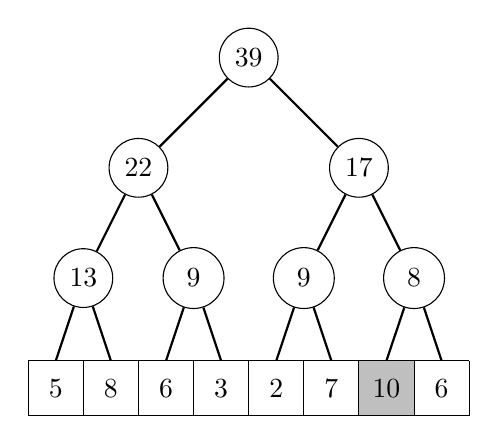
\begin{tikzpicture}[scale=0.7]
\fill[color=lightgray] (6,0) rectangle (7,1);
\draw (0,0) grid (8,1);

\node[anchor=center] at (0.5, 0.5) {5};
\node[anchor=center] at (1.5, 0.5) {8};
\node[anchor=center] at (2.5, 0.5) {6};
\node[anchor=center] at (3.5, 0.5) {3};
\node[anchor=center] at (4.5, 0.5) {2};
\node[anchor=center] at (5.5, 0.5) {7};
\node[anchor=center] at (6.5, 0.5) {10};
\node[anchor=center] at (7.5, 0.5) {6};

\node[draw, circle] (a) at (1,2.5) {13};
\path[draw,thick,-] (a) -- (0.5,1);
\path[draw,thick,-] (a) -- (1.5,1);
\node[draw, circle,minimum size=22pt] (b) at (3,2.5) {9};
\path[draw,thick,-] (b) -- (2.5,1);
\path[draw,thick,-] (b) -- (3.5,1);
\node[draw, circle,minimum size=22pt] (c) at (5,2.5) {9};
\path[draw,thick,-] (c) -- (4.5,1);
\path[draw,thick,-] (c) -- (5.5,1);
\node[draw, circle,minimum size=22pt] (d) at (7,2.5) {8};
\path[draw,thick,-] (d) -- (6.5,1);
\path[draw,thick,-] (d) -- (7.5,1);

\node[draw, circle] (i) at (2,4.5) {22};
\path[draw,thick,-] (i) -- (a);
\path[draw,thick,-] (i) -- (b);
\node[draw, circle] (j) at (6,4.5) {17};
\path[draw,thick,-] (j) -- (c);
\path[draw,thick,-] (j) -- (d);

\node[draw, circle] (m) at (4,6.5) {39};
\path[draw,thick,-] (m) -- (i);
\path[draw,thick,-] (m) -- (j);
\end{tikzpicture}
\end{center}
Actualizamos nodo $14$
\end{frame}

\begin{frame}{Ejemplo de Update}
\begin{center}
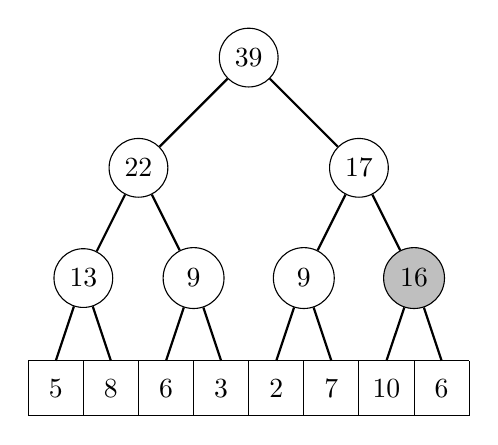
\begin{tikzpicture}[scale=0.7]
\draw (0,0) grid (8,1);

\node[anchor=center] at (0.5, 0.5) {5};
\node[anchor=center] at (1.5, 0.5) {8};
\node[anchor=center] at (2.5, 0.5) {6};
\node[anchor=center] at (3.5, 0.5) {3};
\node[anchor=center] at (4.5, 0.5) {2};
\node[anchor=center] at (5.5, 0.5) {7};
\node[anchor=center] at (6.5, 0.5) {10};
\node[anchor=center] at (7.5, 0.5) {6};

\node[draw, circle] (a) at (1,2.5) {13};
\path[draw,thick,-] (a) -- (0.5,1);
\path[draw,thick,-] (a) -- (1.5,1);
\node[draw, circle,minimum size=22pt] (b) at (3,2.5) {9};
\path[draw,thick,-] (b) -- (2.5,1);
\path[draw,thick,-] (b) -- (3.5,1);
\node[draw, circle,minimum size=22pt] (c) at (5,2.5) {9};
\path[draw,thick,-] (c) -- (4.5,1);
\path[draw,thick,-] (c) -- (5.5,1);
\node[draw, circle,minimum size=22pt, fill=lightgray] (d) at (7,2.5) {16};
\path[draw,thick,-] (d) -- (6.5,1);
\path[draw,thick,-] (d) -- (7.5,1);

\node[draw, circle] (i) at (2,4.5) {22};
\path[draw,thick,-] (i) -- (a);
\path[draw,thick,-] (i) -- (b);
\node[draw, circle] (j) at (6,4.5) {17};
\path[draw,thick,-] (j) -- (c);
\path[draw,thick,-] (j) -- (d);

\node[draw, circle] (m) at (4,6.5) {39};
\path[draw,thick,-] (m) -- (i);
\path[draw,thick,-] (m) -- (j);
\end{tikzpicture}
\end{center}
Actualizamos nodo $7$ $\lfloor14/2\rfloor$
\end{frame}

\begin{frame}{Ejemplo de Update}
\begin{center}
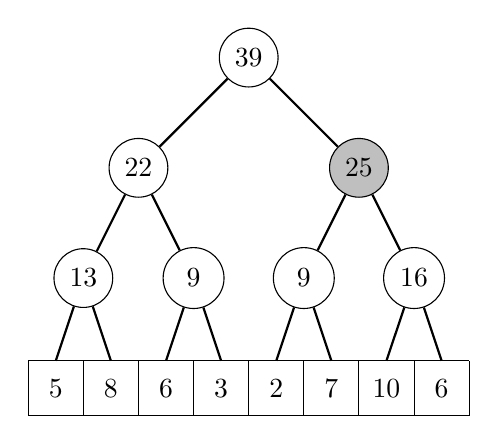
\begin{tikzpicture}[scale=0.7]
\draw (0,0) grid (8,1);

\node[anchor=center] at (0.5, 0.5) {5};
\node[anchor=center] at (1.5, 0.5) {8};
\node[anchor=center] at (2.5, 0.5) {6};
\node[anchor=center] at (3.5, 0.5) {3};
\node[anchor=center] at (4.5, 0.5) {2};
\node[anchor=center] at (5.5, 0.5) {7};
\node[anchor=center] at (6.5, 0.5) {10};
\node[anchor=center] at (7.5, 0.5) {6};

\node[draw, circle] (a) at (1,2.5) {13};
\path[draw,thick,-] (a) -- (0.5,1);
\path[draw,thick,-] (a) -- (1.5,1);
\node[draw, circle,minimum size=22pt] (b) at (3,2.5) {9};
\path[draw,thick,-] (b) -- (2.5,1);
\path[draw,thick,-] (b) -- (3.5,1);
\node[draw, circle,minimum size=22pt] (c) at (5,2.5) {9};
\path[draw,thick,-] (c) -- (4.5,1);
\path[draw,thick,-] (c) -- (5.5,1);
\node[draw, circle,minimum size=22pt] (d) at (7,2.5) {16};
\path[draw,thick,-] (d) -- (6.5,1);
\path[draw,thick,-] (d) -- (7.5,1);

\node[draw, circle] (i) at (2,4.5) {22};
\path[draw,thick,-] (i) -- (a);
\path[draw,thick,-] (i) -- (b);
\node[draw, circle, fill=lightgray] (j) at (6,4.5) {25};
\path[draw,thick,-] (j) -- (c);
\path[draw,thick,-] (j) -- (d);

\node[draw, circle] (m) at (4,6.5) {39};
\path[draw,thick,-] (m) -- (i);
\path[draw,thick,-] (m) -- (j);
\end{tikzpicture}
\end{center}
Actualizamos nodo $3$ $\lfloor7/2\rfloor$
\end{frame}

\begin{frame}{Ejemplo de Update}
\begin{center}
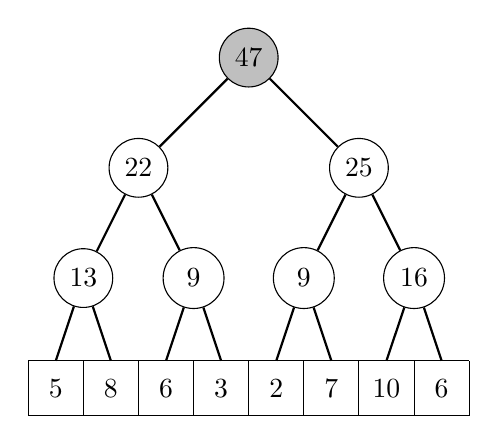
\begin{tikzpicture}[scale=0.7]
\draw (0,0) grid (8,1);

\node[anchor=center] at (0.5, 0.5) {5};
\node[anchor=center] at (1.5, 0.5) {8};
\node[anchor=center] at (2.5, 0.5) {6};
\node[anchor=center] at (3.5, 0.5) {3};
\node[anchor=center] at (4.5, 0.5) {2};
\node[anchor=center] at (5.5, 0.5) {7};
\node[anchor=center] at (6.5, 0.5) {10};
\node[anchor=center] at (7.5, 0.5) {6};

\node[draw, circle] (a) at (1,2.5) {13};
\path[draw,thick,-] (a) -- (0.5,1);
\path[draw,thick,-] (a) -- (1.5,1);
\node[draw, circle,minimum size=22pt] (b) at (3,2.5) {9};
\path[draw,thick,-] (b) -- (2.5,1);
\path[draw,thick,-] (b) -- (3.5,1);
\node[draw, circle,minimum size=22pt] (c) at (5,2.5) {9};
\path[draw,thick,-] (c) -- (4.5,1);
\path[draw,thick,-] (c) -- (5.5,1);
\node[draw, circle,minimum size=22pt] (d) at (7,2.5) {16};
\path[draw,thick,-] (d) -- (6.5,1);
\path[draw,thick,-] (d) -- (7.5,1);

\node[draw, circle] (i) at (2,4.5) {22};
\path[draw,thick,-] (i) -- (a);
\path[draw,thick,-] (i) -- (b);
\node[draw, circle] (j) at (6,4.5) {25};
\path[draw,thick,-] (j) -- (c);
\path[draw,thick,-] (j) -- (d);

\node[draw, circle, fill=lightgray] (m) at (4,6.5) {47};
\path[draw,thick,-] (m) -- (i);
\path[draw,thick,-] (m) -- (j);
\end{tikzpicture}
\end{center}
Actualizamos nodo $1$ $\lfloor3/2\rfloor$
\end{frame}

\subsection{Código}

\begin{frame}[fragile]{Version Iterativa}
\begin{lstlisting}
int retrieve(int a, int b) {
    a += n; b += n;
    int s = 0;
    while (a <= b) {
        if (a%2 == 1) s += tree[a++];
        if (b%2 == 0) s += tree[b--];
        a /= 2; b /= 2;
    }
    return s;
}

void update(int k, int x) {
    k += n, tree[k] += x;
    for (k /= 2; k >= 1; k /= 2) {
        tree[k] = tree[2*k]+tree[2*k+1];
    }
}
\end{lstlisting}
\end{frame}

\begin{frame}[fragile]{Version Recursiva}
\begin{lstlisting}
int sum(int a, int b, int k, int x, int y) {
    if (b < x || a > y) return 0;
    if (a <= x && y <= b) return tree[k];
    int d = (x+y)/2;
    return sum(a,b,2*k,x,d) + sum(a,b,2*k+1,d+1,y);
}
      
void update(int pos, int k, int x, int y, int val) {
    if (x == y) { segTree[k] = val; return; }
    int d = (x + y) / 2;
    if (pos <= d) update(pos, k*2, x, d, val);
    else update(pos, k*2+1, d+1, y, val);
    segTree[k] = segTree[k*2] + segTree[k*2+1];
}

\end{lstlisting}
\end{frame}

\subsection{Complejidad}

\begin{frame}{Complejidad}
\begin{itemize}
    \item Construcción: $O(n)$ (De todas formas, solemos construirlo usando la operación update)
    \item Query: $O(log\:n)$
    \item Update: $O(log\:n)$
    \item Memoria: $O(2n)$
\end{itemize}
Puede notarse que el árbol que construimos es un árbol binario completo, por lo que la cantidad de nodos es $2n-1$, y tiene una profundidad de $log_2(n)$.
\end{frame}

\begin{frame}{Entendiendo la Complejidad de Query}
Es fácil creer que la complejidad de query es mayor a $O(log\:n)$, ya que en cada nivel del árbol se podría llamar a los dos nodos hijos. Pero, en total, notemos que en cada nivel solo se van a estar llamando como máximo $4$ nodos en su versión recursiva, y $2$ en la versión iterativa. Veamos el caso recursivo, que es el más confuso.

\begin{itemize}
    \item El nodo está afuera del rango: no se llama a ningún hijo.
    \item El nodo está completamente dentro del rango: no se llama a ningún hijo.
    \item El nodo está parcialmente dentro del rango: se llama a los dos hijos. Esto puede ocurrir hasta dos veces por paso, ya que el intervalo es contiguo.
\end{itemize}
\end{frame}

\subsection{Resolución de un Problema}

\begin{frame}{Resolución del Problema}
Veamos el Código de "Dynamic Range Sum Queries".

\url{https://cses.fi/problemset/task/1648}
\end{frame}

\section{Generalización del Segment Tree}

\begin{frame}{Pregunta Motivadora}
La estructura de datos que trabajamos anteriormente, ¿sólo nos permite trabajar con la suma?

\pause
¡No! Podemos generalizarla para cualquier operación que sea asociativa y tenga un elemento neutro. A este tipo de operaciones las llamamos \textbf{monoides}.
\end{frame}

\subsection{Monoides}

\begin{frame}{Definición de Monoide}
Un Monoide es una estructura algebraica con una operación binaria, que es asociativa y tiene elemento neutro. Un Monoide se lo puede denotar como $(A, \oplus)$ y en lenguaje formal se define como:
\begin{itemize}
    \item $\forall a,b,c \in A, (a \oplus b) \oplus c = a \oplus (b \oplus c)$ (es asociativa)
    \item $\exists !e \in A, \forall a \in A, a \oplus e = e \oplus a = a$ (existe neutro)
    \item $\forall a,b \in A, a \oplus b \in A$ (operación cerrada)
\end{itemize}
\end{frame}

\begin{frame}{Ejemplos de Monoide}
Estos son algunos ejemolos de Monoides, que pueden ser interesantes para resolver problemas de Programación Competitiva:
\begin{itemize}
    \item $(\mathbb{N}, +)$
    \item $(\mathbb{N}, \times)$
    \item $(\mathbb{N}, min)$
    \item $(\mathbb{N}, max)$
    \item $(\mathbb{N}, gcd)$
    \item $(\mathbb{N}, lcm)$
    \item $(\mathbb{N}, \land)$
    \item $(\mathbb{N}, \lor)$
    \item $(\mathbb{N}, \oplus)$, donde $\oplus$ es el XOR
    \item $(\text{string}, +)$, donde $+$ es la concatenación
\end{itemize}
\end{frame}

\subsection{Implementación Generalizada del Segment Tree}

\begin{frame}{Implementación Generalizada}
Ahora, vamos a ver en C++ una implementación generalizada del Segment Tree, que nos permita trabajar con cualquier Monoide. Esta idea es gran cortesía de Tarche, que hizo que esté en nuestro Notebook para ICPC.
\end{frame}

\subsection{Resolviendo Más Problemas}
\begin{frame}{Resolviendo Más Problemas}
Resolvamos los siguientes problemas de CSES con la implementación de Monoide:
\begin{itemize}
    \item \url{https://cses.fi/problemset/task/1649}
    \item \url{https://cses.fi/problemset/task/1650}
\end{itemize}
\end{frame}

\section{Más Problemas de Segment Tree}

\subsection{Hotel Queries}
\begin{frame}{Hotel Queries}
\begin{block}{CSES 1143 - Hotel Queries}
Hay $n$ hoteles en una calle. Para cada hotel conoces el número de habitaciones libres. Tu tarea es asignar habitaciones de hotel para grupos de turistas. Todos los miembros de un grupo quieren alojarse en el mismo hotel.

Los grupos llegarán a usted uno tras otro y usted sabrá para cada grupo la cantidad de habitaciones que necesita. Siempre asignas un grupo al primer hotel que tenga suficientes habitaciones. Después de esto, el número de habitaciones libres en el hotel disminuye.

Para cada grupo de turistas, imprima el número del hotel al que fueron asignados.
\end{block}

\url{https://cses.fi/problemset/task/1143}
\end{frame}

\begin{frame}{Recorriendo Alternativamente el Segment Tree}
Para resolver el problema, vamos a usar el Segment Tree de máximos como una estructura para hacer Binary Search. La idea es encontrar el primer hotel que tenga suficientes habitaciones para el grupo de turistas en $O(log \text{ } n)$.

\pause
Partimos del primer nodo (la raíz), y recorremos el de la izquierda si el nodo contiene un número mayor o igual a la cantidad de habitaciones que necesitamos, o el de la derecha si el nodo contiene un número menor.

\pause
Luego, actualizamos el Segment Tree para que tenga menos habitaciones libres. ¡Veamos el código!
\end{frame}

\end{document}

% Bibliografía: https://cses.fi/book/book.pdf, http://www.oia.unsam.edu.ar/wp-content/uploads/2017/11/segment-tree.pdf, https://es.wikipedia.org/wiki/Monoide
